\documentclass[11pt]{article}

\usepackage[margin=0.82in]{geometry}
\usepackage[T1]{fontenc}
\usepackage[utf8]{inputenc}
\usepackage{lmodern}
\usepackage{microtype}
\usepackage{xcolor}
\usepackage{graphicx}
\usepackage{amsmath}
\usepackage{booktabs}
\usepackage{tabularx}
\usepackage{array}
\usepackage{enumitem}
\usepackage{float}
\usepackage{hyperref}
\usepackage{tikz}
\usetikzlibrary{arrows.meta, positioning, shapes.geometric, calc, fit, backgrounds}
\graphicspath{{figures/}{../figures/}}

\definecolor{Ink}{HTML}{16212B}
\definecolor{Muted}{HTML}{5D6B73}
\definecolor{Blue}{HTML}{2563EB}
\definecolor{Teal}{HTML}{0F766E}
\definecolor{Green}{HTML}{15803D}
\definecolor{Amber}{HTML}{B7791F}
\definecolor{Red}{HTML}{B91C1C}
\definecolor{Panel}{HTML}{F5F7FA}
\definecolor{Line}{HTML}{CAD5E2}
\definecolor{SoftBlue}{HTML}{DBEAFE}
\definecolor{SoftTeal}{HTML}{CCFBF1}
\definecolor{SoftGreen}{HTML}{DCFCE7}
\definecolor{SoftAmber}{HTML}{FEF3C7}
\definecolor{SoftRed}{HTML}{FEE2E2}

\hypersetup{
  colorlinks=true,
  linkcolor=Blue,
  urlcolor=Teal,
  citecolor=Blue
}

\setlength{\parindent}{0pt}
\setlength{\parskip}{0.58em}
\setlist[itemize]{leftmargin=1.4em, topsep=0.25em, itemsep=0.12em}
\setlist[enumerate]{leftmargin=1.6em, topsep=0.25em, itemsep=0.12em}
\renewcommand{\arraystretch}{1.18}

\newcolumntype{Y}{>{\raggedright\arraybackslash}X}
\newcommand{\tagbox}[2]{%
  \tikz[baseline=(n.base)] \node[rounded corners=2pt, fill=#1, inner xsep=5pt, inner ysep=2pt] (n) {\footnotesize #2};%
}

\title{\vspace{-1.4cm}\textbf{From Manual Benchwork to Data-Producing Robotic Laboratories}\\
\large A Feasibility Roadmap for Dexterous Automation in Experimental Workflows}
\author{Strategic Technical Brief}
\date{\today}

\begin{document}
\maketitle
\vspace{-0.8em}

\begin{abstract}
Robotic laboratory automation is technically feasible, but its near-term value will not come from a fully general ``dark laboratory'' on day one. The practical path is to choose a narrow, repetitive, economically meaningful workflow, redesign that workflow around robot-friendly primitives, and use the system to generate standardized experimental data at scale. The strongest initial wedge is a semi-standardized biological or biochemical screening workflow where liquid handling, media exchange, plate movement, imaging/readout, and condition exploration can be converted into repeatable robot actions. A dexterous hand is useful, but the first product should be a complete task cell: mobile or fixed base, arm, end-effector, vision, optional tactile sensing, scheduling software, and a data layer.
\end{abstract}

\section{Executive Conclusion}

The feasible strategy is not to imitate a human researcher in every operation. The feasible strategy is to industrialize a constrained class of experiments. A first system should solve one high-frequency task family, collect every action and result as structured data, and prove an economic case that is visible within a two-year decision window.

\textbf{Recommended wedge.} Start with a robot-ready screening and maintenance workflow: stock-solution preparation, liquid transfer, plate/culture maintenance, media exchange, standardized imaging/readout, and data capture. Avoid early dependence on highly nonstandard tissue handling, powder weighing with extreme precision, or general-purpose manipulation across many unrelated laboratory contexts.

\textbf{Recommended architecture.} Use a wheeled or fixed laboratory workcell with arm-plus-dexterous-end-effector, side or wrist vision, optional tactile sensing for contact-rich steps, and a workflow layer that converts protocols into robot-executable primitives. Tendon-driven hands are attractive for long-term reliability and impact tolerance, while direct-drive hands remain useful for low-cost prototyping and simple demonstrations.

\textbf{Recommended commercialization path.} Sell outcomes first, not components. The customer should buy validated runs, structured datasets, or a complete automated task cell, rather than a bare robotic hand that requires deep integration work.

\begin{figure}[htbp]
\centering
\includegraphics[width=\linewidth]{aginti_lab_workcell.png}
\caption{A complete workcell links planning, manipulation, sensing, instruments, data storage, and quality feedback into a single operational system.}
\label{fig:workcell-overview}
\end{figure}

\begin{figure}[htbp]
\centering
\resizebox{\linewidth}{!}{%
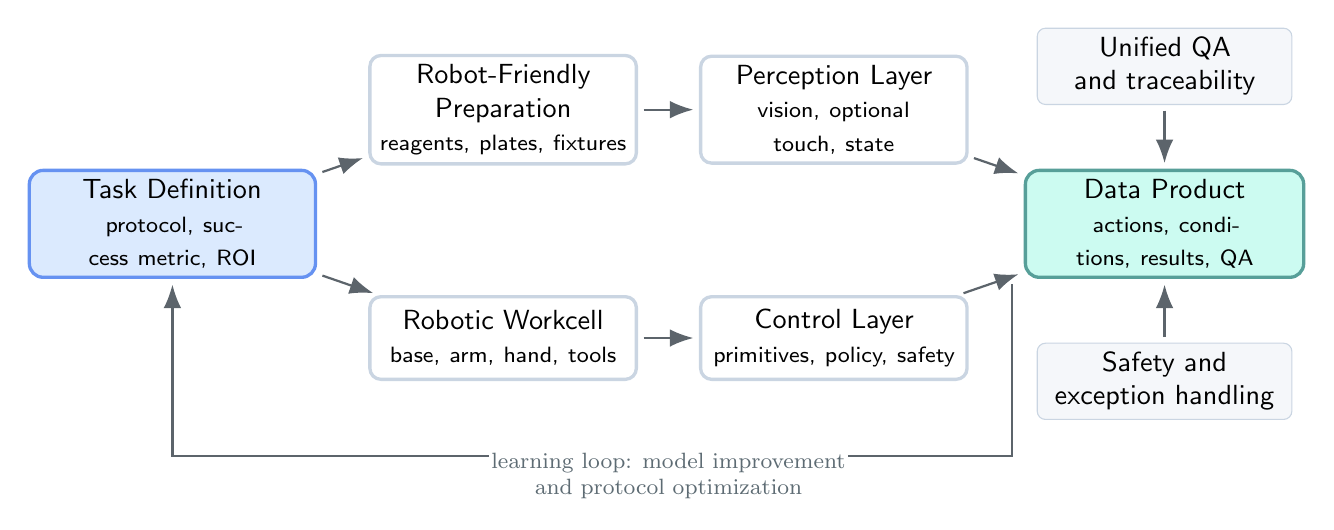
\begin{tikzpicture}[
  font=\sffamily,
  box/.style={rounded corners=4pt, draw=Line, very thick, fill=white, align=center, text width=3.15cm, minimum height=1.05cm},
  core/.style={rounded corners=5pt, draw=Blue!70, very thick, fill=SoftBlue, align=center, text width=3.4cm, minimum height=1.1cm},
  data/.style={rounded corners=5pt, draw=Teal!70, very thick, fill=SoftTeal, align=center, text width=3.3cm, minimum height=1.1cm},
  arrow/.style={-{Latex[length=3mm]}, thick, draw=Ink!70, shorten >=2pt, shorten <=2pt},
  note/.style={rounded corners=3pt, fill=Panel, draw=Line, align=center, text width=3.0cm, minimum height=0.8cm}
]
\node[core] (task) at (0,0) {Task Definition\\\footnotesize protocol, success metric, ROI};
\node[box] (prep) at (4.2,1.45) {Robot-Friendly\\Preparation\\\footnotesize reagents, plates, fixtures};
\node[box] (robot) at (4.2,-1.45) {Robotic Workcell\\\footnotesize base, arm, hand, tools};
\node[box] (sense) at (8.4,1.45) {Perception Layer\\\footnotesize vision, optional touch, state};
\node[box] (control) at (8.4,-1.45) {Control Layer\\\footnotesize primitives, policy, safety};
\node[data] (data) at (12.6,0) {Data Product\\\footnotesize actions, conditions, results, QA};

\draw[arrow] (task) -- (prep);
\draw[arrow] (task) -- (robot);
\draw[arrow] (prep) -- (sense);
\draw[arrow] (robot) -- (control);
\draw[arrow] (sense) -- (data);
\draw[arrow] (control) -- (data);
\draw[arrow] ([xshift=-0.15cm]data.south west) -- ++(0,-2.25) -| (task.south);
\node[font=\footnotesize\color{Muted}, align=center, fill=white, inner sep=1pt] at (6.3,-3.2) {learning loop: model improvement\\and protocol optimization};

\node[note] (qa) at (12.6,2.0) {Unified QA\\and traceability};
\draw[arrow] (qa) -- (data);
\node[note] (safety) at (12.6,-2.0) {Safety and\\exception handling};
\draw[arrow] (safety) -- (data);
\end{tikzpicture}}
\caption{A practical robotic laboratory should be treated as a complete data-producing workcell, not as an isolated robotic hand.}
\label{fig:architecture}
\end{figure}

\section{Technical Premise}

Robotic manipulation for laboratory work sits between two extremes. A fully general humanoid laboratory worker is attractive but expensive, integration-heavy, and unlikely to be product-ready in the near term. A narrow liquid-handler is mature but cannot address many workflows that remain manual because they require grasping, repositioning, force modulation, tool use, or ad hoc interaction with existing bench instruments.

The opportunity is the middle layer: dexterous robotic workcells that can handle a selected family of protocols while the environment is simplified enough to make the manipulation problem tractable.

\subsection*{Direct-drive and tendon-driven hands}

\begin{table}[htbp]
\centering
\small
\begin{tabularx}{\linewidth}{@{}p{3.0cm}YY@{}}
\toprule
\textbf{Dimension} & \textbf{Direct-drive hand} & \textbf{Tendon-driven hand} \\
\midrule
Near-term advantage & Lower integration cost; simpler demonstration; more mature component availability. & Better ceiling for impact tolerance, remote motor placement, thermal isolation, and long-duration operation. \\
Main weakness & Heat, impact transmission, motor/gear wear, and tactile drift near the fingers. & Harder control problem; higher software and integration burden. \\
Best use & Prototyping, simple grasping, preprogrammed demonstrations, low-cost SDK experimentation. & Production-oriented laboratory workcells requiring repeated contact, tactile feedback, and reliable long-running operation. \\
Strategic role & Learning vehicle and entry-level product. & Long-term platform for robust laboratory automation. \\
\bottomrule
\end{tabularx}
\caption{A staged strategy can use direct-drive hardware for learning while reserving tendon-driven designs for higher-reliability workcells.}
\label{tab:drive}
\end{table}

\section{Where to Start}

The first workflow must be chosen by task economics, not by technical ambition. A good starting task should satisfy five conditions:

\begin{enumerate}
  \item It is repeated often enough that automation produces visible value.
  \item It can be standardized through fixtures, prepared reagents, plates, carriers, or simplified protocols.
  \item It generates useful structured data, not merely labor savings.
  \item It avoids fragile edge cases in the first version.
  \item It can be demonstrated with a measurable baseline against human operation or existing outsourced workflows.
\end{enumerate}

\begin{figure}[htbp]
\centering
\resizebox{0.96\linewidth}{!}{%
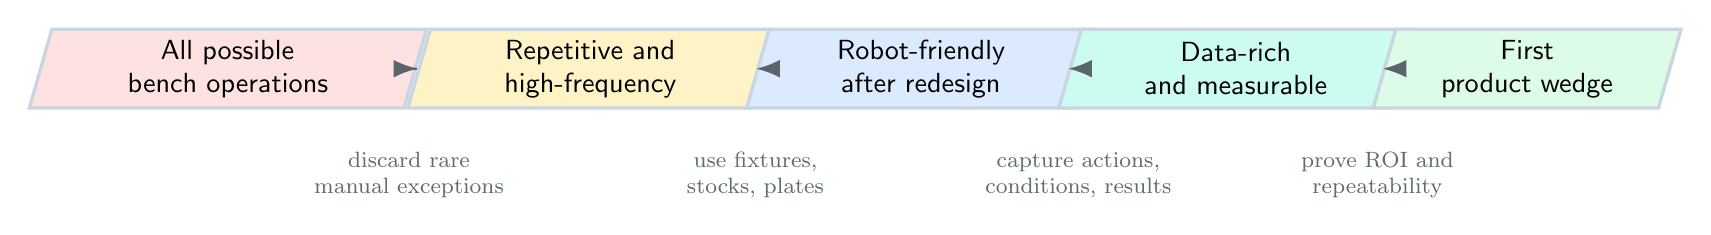
\begin{tikzpicture}[
  font=\sffamily,
  stage/.style={trapezium, trapezium left angle=74, trapezium right angle=106, draw=Line, very thick, align=center, minimum height=1.0cm},
  arrow/.style={-{Latex[length=3mm]}, thick, draw=Ink!70},
  label/.style={font=\footnotesize\color{Muted}, align=center}
]
\node[stage, fill=SoftRed, text width=4.1cm] (s1) at (0,0) {All possible\\bench operations};
\node[stage, fill=SoftAmber, text width=3.7cm] (s2) at (4.6,0) {Repetitive and\\high-frequency};
\node[stage, fill=SoftBlue, text width=3.5cm] (s3) at (8.8,0) {Robot-friendly\\after redesign};
\node[stage, fill=SoftTeal, text width=3.3cm] (s4) at (12.8,0) {Data-rich\\and measurable};
\node[stage, fill=SoftGreen, text width=3.0cm] (s5) at (16.5,0) {First\\product wedge};

\draw[arrow] (s1) -- (s2);
\draw[arrow] (s2) -- (s3);
\draw[arrow] (s3) -- (s4);
\draw[arrow] (s4) -- (s5);

\node[label] at (2.3,-1.35) {discard rare\\manual exceptions};
\node[label] at (6.7,-1.35) {use fixtures,\\stocks, plates};
\node[label] at (10.8,-1.35) {capture actions,\\conditions, results};
\node[label] at (14.6,-1.35) {prove ROI and\\repeatability};
\end{tikzpicture}}
\caption{The first product should pass through a task-selection funnel before any hardware commitment.}
\label{fig:funnel}
\end{figure}

\subsection*{Promising first workflows}

{\footnotesize
\begin{tabularx}{\linewidth}{@{}>{\raggedright\arraybackslash}p{2.8cm}>{\raggedright\arraybackslash}p{1.25cm}Y>{\raggedright\arraybackslash}p{4.0cm}@{}}
\toprule
\textbf{Workflow} & \textbf{Fit} & \textbf{Reason} & \textbf{First milestone} \\
\midrule
Cell-culture media exchange & High & Repetitive, disliked, schedule-sensitive, and close to standard liquid handling. & Run one plate format with contamination and viability tracking. \\
Stock-solution preparation & High & Converts difficult powder handling into easier liquid workflows and lowers manipulation precision requirements. & Prepare reagents with mass/volume traceability and error checks. \\
Assay screening and imaging & High & Produces structured, monetizable datasets; aligns with pharmaceutical discovery workflows. & Complete one plate run with condition metadata, imaging output, and QC report. \\
Organoid or tissue maintenance & Medium & High value but less standardized; should follow after simpler 2D or 2.5D protocols. & Pilot one standardized organoid format. \\
General laboratory chores & Low & Too broad, weak ROI, and high variation. & Defer until task cell primitives are mature. \\
\bottomrule
\end{tabularx}
}

\section{Product Concept}

The first deployable product should be a \textbf{Robotic Assay Workcell}. It should not claim general laboratory autonomy. It should claim reliable execution of a bounded workflow with traceable data.

\textbf{Hardware.} A fixed bench cell is the simplest starting point. A wheeled base becomes useful when the system must move among instruments, but fixed installations reduce navigation complexity. A hand-plus-arm configuration is sufficient for early versions; humanoid legs are unnecessary in laboratories and introduce avoidable safety risks around expensive instruments.

\textbf{Sensing.} Vision should be included by default. Tactile sensing should be added only for contact-rich steps where force, slip, or insertion feedback materially improves success. For simple scripted gestures, tactile feedback is unnecessary; for real laboratory interaction, multimodal feedback becomes important.

\textbf{Control.} The system should combine low-level SDK control, guarded motion primitives, visual state estimation, and a learned policy only where variation requires adaptation. A fully learned controller should not be the first dependency for every action.

\begin{figure}[htbp]
\centering
\resizebox{\linewidth}{!}{%
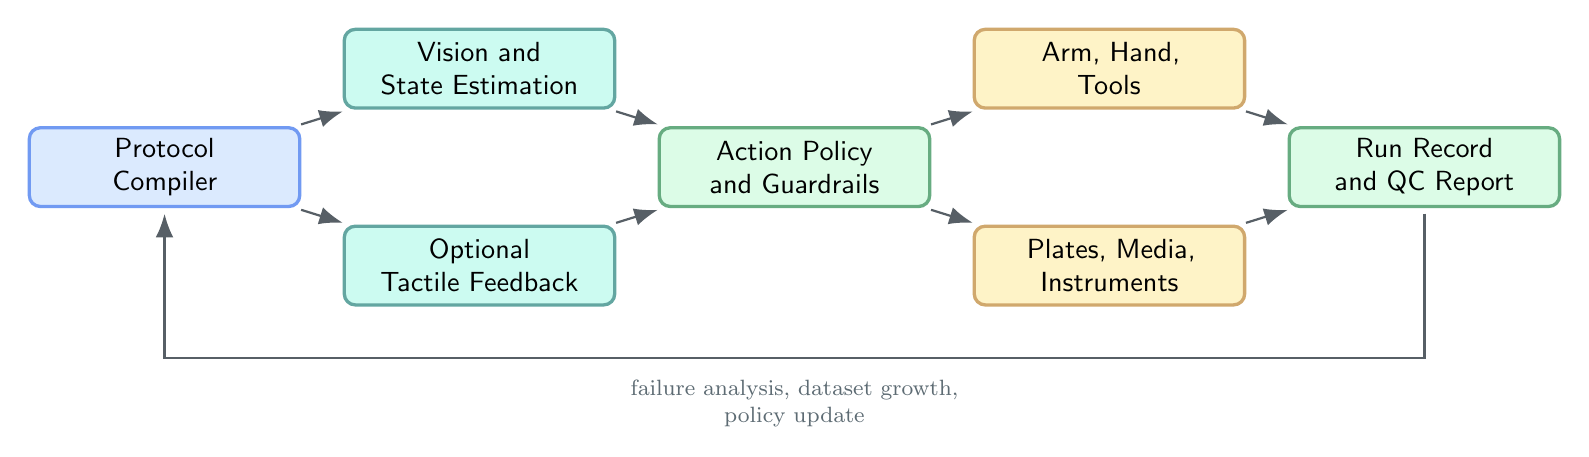
\begin{tikzpicture}[
  font=\sffamily,
  block/.style={rounded corners=4pt, draw=Line, very thick, fill=white, align=center, text width=3.2cm, minimum height=1.0cm},
  blue/.style={block, fill=SoftBlue, draw=Blue!65},
  teal/.style={block, fill=SoftTeal, draw=Teal!65},
  green/.style={block, fill=SoftGreen, draw=Green!65},
  amber/.style={block, fill=SoftAmber, draw=Amber!65},
  arrow/.style={-{Latex[length=3mm]}, thick, draw=Ink!72, shorten >=2pt, shorten <=2pt}
]
\node[blue] (proto) at (0,0) {Protocol\\Compiler};
\node[teal] (state) at (4.0,1.25) {Vision and\\State Estimation};
\node[teal] (touch) at (4.0,-1.25) {Optional\\Tactile Feedback};
\node[green] (policy) at (8.0,0) {Action Policy\\and Guardrails};
\node[amber] (robot) at (12.0,1.25) {Arm, Hand,\\Tools};
\node[amber] (lab) at (12.0,-1.25) {Plates, Media,\\Instruments};
\node[green] (qa) at (16.0,0) {Run Record\\and QC Report};

\draw[arrow] (proto) -- (state);
\draw[arrow] (proto) -- (touch);
\draw[arrow] (state) -- (policy);
\draw[arrow] (touch) -- (policy);
\draw[arrow] (policy) -- (robot);
\draw[arrow] (policy) -- (lab);
\draw[arrow] (robot) -- (qa);
\draw[arrow] (lab) -- (qa);
\draw[arrow] (qa.south) -- ++(0,-1.9) -| (proto.south);
\node[font=\footnotesize\color{Muted}, align=center, fill=white, inner sep=1pt] at (8.0,-3.0) {failure analysis, dataset growth,\\policy update};
\end{tikzpicture}}
\caption{The control stack should turn protocols into guarded robot actions and structured data, with feedback loops for continuous improvement.}
\label{fig:control}
\end{figure}

\section{Economic Logic}

The commercial case should be framed around three value pools:

\begin{itemize}
  \item \textbf{Labor substitution:} fewer repetitive manual operations, fewer night/weekend shifts, and less dependence on operator consistency.
  \item \textbf{Facility leverage:} experiments can move toward lower-cost, high-throughput facilities while researchers remain close to planning and analysis.
  \item \textbf{Data production:} the system generates standardized action-condition-result datasets that may become more valuable than the robotic operation itself.
\end{itemize}

The strongest business model is not simply selling hardware. It is selling validated experimental runs, datasets, or a managed workcell with service-level commitments. A hardware-only sale transfers too much integration risk to the customer and makes support difficult.

\[
\text{Adoption pressure} =
\frac{\text{visible cost saving} + \text{data value} + \text{safety value}}
{\text{integration burden} + \text{workflow disruption} + \text{technical risk}}
\]

The numerator must be proven early. Customers with mature teams and existing outsourcing channels will not change workflows unless the benefit is immediate, measurable, and large enough to offset disruption.

\section{Roadmap}

\begin{figure}[H]
\centering
\resizebox{\linewidth}{!}{%
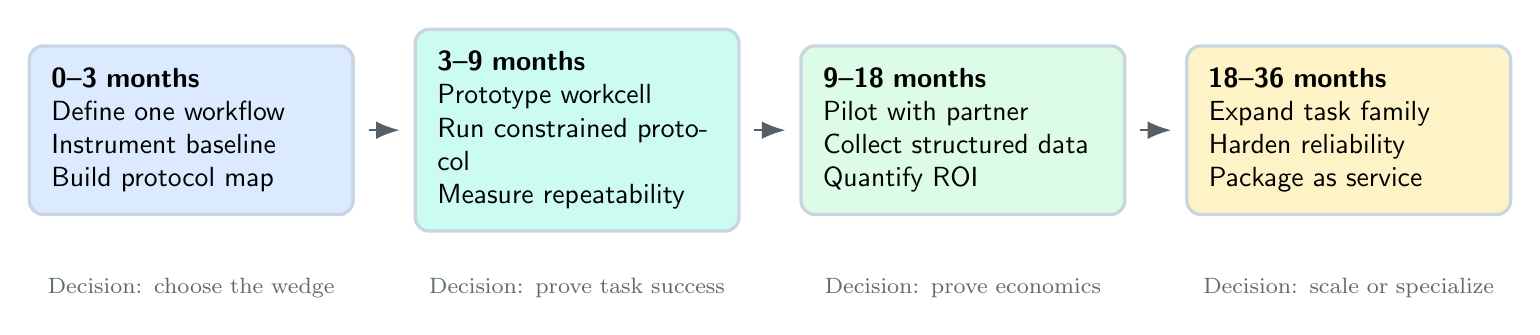
\begin{tikzpicture}[
  font=\sffamily,
  phase/.style={rounded corners=5pt, draw=Line, very thick, fill=white, align=left, text width=3.55cm, minimum height=2.1cm, inner sep=8pt},
  arrow/.style={-{Latex[length=3mm]}, thick, draw=Ink!72, shorten >=5pt, shorten <=5pt}
]
\node[phase, fill=SoftBlue] (p1) at (0,0) {\textbf{0--3 months}\\Define one workflow\\Instrument baseline\\Build protocol map};
\node[phase, fill=SoftTeal] (p2) at (4.9,0) {\textbf{3--9 months}\\Prototype workcell\\Run constrained protocol\\Measure repeatability};
\node[phase, fill=SoftGreen] (p3) at (9.8,0) {\textbf{9--18 months}\\Pilot with partner\\Collect structured data\\Quantify ROI};
\node[phase, fill=SoftAmber] (p4) at (14.7,0) {\textbf{18--36 months}\\Expand task family\\Harden reliability\\Package as service};

\draw[arrow] (p1) -- (p2);
\draw[arrow] (p2) -- (p3);
\draw[arrow] (p3) -- (p4);

\node[font=\footnotesize\color{Muted}, align=center, text width=3.9cm] at (0,-2.0) {Decision: choose the wedge};
\node[font=\footnotesize\color{Muted}, align=center, text width=3.9cm] at (4.9,-2.0) {Decision: prove task success};
\node[font=\footnotesize\color{Muted}, align=center, text width=3.9cm] at (9.8,-2.0) {Decision: prove economics};
\node[font=\footnotesize\color{Muted}, align=center, text width=3.9cm] at (14.7,-2.0) {Decision: scale or specialize};
\end{tikzpicture}}
\caption{A realistic commercialization timeline should treat full laboratory autonomy as a multi-year program, while still delivering useful pilots early.}
\label{fig:roadmap}
\end{figure}

\subsection*{Immediate actions}

\begin{enumerate}
  \item \textbf{Select one protocol.} Pick a task such as cell media exchange plus assay readout, stock-solution preparation plus plate dosing, or standardized organoid screening. Do not start with a broad laboratory assistant.
  \item \textbf{Write the task contract.} Define inputs, outputs, acceptable error, contamination threshold, throughput, run time, and what counts as failure.
  \item \textbf{Redesign the environment.} Use fixtures, carriers, standardized containers, preprepared liquids, and instrument placement that simplify robot motion.
  \item \textbf{Build a baseline.} Measure current human or outsourced cost, cycle time, variance, failure rate, and data quality.
  \item \textbf{Prototype the minimum workcell.} Combine arm, hand/tool, vision, motion primitives, and a run logger. Add tactile sensing only when a step requires it.
  \item \textbf{Generate a first dataset.} The first milestone is not only task completion; it is a traceable dataset that ties protocol conditions to outcomes.
  \item \textbf{Decide by economics.} Continue only if the system can show a credible path to lower cost, better consistency, safer operation, or valuable data production.
\end{enumerate}

\section{Risks and Mitigations}

\begin{tabularx}{\linewidth}{@{}p{3.1cm}YY@{}}
\toprule
\textbf{Risk} & \textbf{Failure mode} & \textbf{Mitigation} \\
\midrule
Over-generalization & The product becomes a vague laboratory humanoid project with no measurable first customer. & Constrain the first release to one protocol and one environment. \\
Manipulation difficulty & Powder handling, deformable tissue, or fragile instruments create too many edge cases. & Convert powders to stock solutions, use fixtures, and defer highly nonstandard handling. \\
Sensor drift & Heat, wear, and tactile inconsistency reduce reliability over long runs. & Prefer remote actuation where useful, track calibration, and use tactile sensing selectively. \\
Integration burden & Customers need custom engineering for every deployment. & Sell a complete task cell or managed service, not a bare hand. \\
Weak ROI & The system is technically impressive but not economically compelling. & Measure labor, facility, safety, data, and failure costs before building the pilot. \\
Data disorder & Automated runs produce volume without usable metadata. & Make run logging and schema design part of the first prototype. \\
\bottomrule
\end{tabularx}

\section{Feasible First Demonstration}

A strong first demonstration would show a robot executing a bounded screen:

\begin{enumerate}
  \item prepare or receive standardized stock solutions;
  \item dose plates or culture vessels under a known protocol;
  \item perform scheduled media exchange or maintenance;
  \item move samples to imaging or readout;
  \item record conditions, actions, errors, images, and results;
  \item generate a QC report and a dataset ready for analysis.
\end{enumerate}

This demonstration is narrow enough to be feasible and broad enough to support a larger story: laboratories can shift from manual execution to data-producing experimental infrastructure. In that model, the operator designs experiments and reviews results, while the robotic cell executes repeatable work and creates standardized data around the clock.

\section{Bottom Line}

The most credible path is a staged automation program. The first stage should not promise complete human replacement. It should prove that a robot-friendly protocol can run repeatably, safely, and economically while producing structured data. Once that foundation works, the platform can expand from one task to a family of experimental workflows, and eventually toward distributed, lower-cost, high-throughput laboratories.

\end{document}
